% CSE 715 — Computer Graphics
% Chapter 3: Scan Conversion — Complete Model Answers (2020–2024)
% University of Chittagong, 7th Semester B.Sc. Engineering
% Source: Schaum's Outline of Computer Graphics (Xiang & Plastock), Chapter 3, pp.25-67
%
% Compile with: pdflatex Chapter3_Solutions.tex (run twice for TOC)

\documentclass[12pt, a4paper]{article}

\usepackage[left=2.5cm, right=2.5cm, top=2.8cm, bottom=2.8cm, headheight=15pt]{geometry}
\usepackage{amsmath, amssymb}
\usepackage{tikz}
\usetikzlibrary{arrows.meta, positioning, shapes.geometric, calc, backgrounds, fit}
\usepackage{booktabs}
\usepackage{array}
\usepackage{xcolor}
\usepackage{enumitem}
\usepackage{fancyhdr}
\usepackage{titlesec}
\usepackage{mdframed}
\usepackage{multicol}
\usepackage{tabularx}
\usepackage{multirow}
\usepackage{hyperref}

%----- Colours -----
\definecolor{sectionblue}{RGB}{10,60,110}
\definecolor{boxbg}{RGB}{242,247,255}
\definecolor{answerbg}{RGB}{240,255,240}
\definecolor{notesbg}{RGB}{255,250,230}
\definecolor{keyblue}{RGB}{0,80,160}
\definecolor{accent}{RGB}{180,40,40}

%----- Box environments -----
\mdfdefinestyle{solutionframe}{linecolor=sectionblue, backgroundcolor=boxbg, roundcorner=4pt, linewidth=1.4pt, innertopmargin=7pt, innerbottommargin=7pt, innerleftmargin=9pt, innerrightmargin=9pt}
\mdfdefinestyle{answerframe}{linecolor=green!55!black, backgroundcolor=answerbg, roundcorner=4pt, linewidth=1.4pt, innertopmargin=7pt, innerbottommargin=7pt, innerleftmargin=9pt, innerrightmargin=9pt}
\mdfdefinestyle{notesframe}{linecolor=orange!70!black, backgroundcolor=notesbg, roundcorner=4pt, linewidth=1pt, innertopmargin=5pt, innerbottommargin=5pt, innerleftmargin=8pt, innerrightmargin=8pt}
\newenvironment{solutionbox}{\begin{mdframed}[style=solutionframe]}{\end{mdframed}}
\newenvironment{answerbox}{\begin{mdframed}[style=answerframe]}{\end{mdframed}}
\newenvironment{notesbox}{\begin{mdframed}[style=notesframe]}{\end{mdframed}}

%----- Page style -----
\pagestyle{fancy}
\fancyhf{}
\lhead{\small\color{sectionblue} CSE 715 --- Chapter 3: Scan Conversion}
\rhead{\small\color{sectionblue} Model Solutions (2020--2024)}
\cfoot{\small\thepage}
\renewcommand{\headrulewidth}{0.5pt}

%----- Section formatting -----
\titleformat{\section}{\Large\bfseries\color{sectionblue}}{}{0em}{}[\vspace{-2pt}\color{sectionblue}\rule{\linewidth}{0.8pt}]
\titleformat{\subsection}{\large\bfseries\color{sectionblue!85!black}}{}{0em}{}
\titleformat{\subsubsection}{\normalsize\bfseries\color{black}}{}{0em}{}

%----- Custom list -----
\newlist{keypoints}{itemize}{1}
\setlist[keypoints]{label=$\triangleright$, leftmargin=1.5cm, itemsep=2pt, topsep=3pt}
\newlist{examlist}{enumerate}{1}
\setlist[examlist]{label=\textbf{(\roman*)}, leftmargin=1.8cm, itemsep=3pt, topsep=4pt}

%=====================================================================
\begin{document}
%=====================================================================

\begin{center}
  {\LARGE\bfseries\color{sectionblue} CSE 715: Computer Graphics}\\[0.6em]
  {\Large\bfseries Chapter 3 --- Scan Conversion}\\[0.3em]
  {\large Complete Model Answers (2020--2024)}\\[0.2em]
  {\normalsize University of Chittagong \quad|\quad 7\textsuperscript{th} Semester B.Sc.\ (Engg.) Examination}\\[0.3em]
  {\small Source: Schaum's Outline of Computer Graphics (Xiang \& Plastock), Chapter 3, pp.25--67}
\end{center}

\vspace{0.3em}
\noindent\rule{\linewidth}{1pt}
\vspace{0.5em}

\tableofcontents
\newpage

%=====================================================================
\section{Theoretical Framework --- Reusable Across All Years}
%=====================================================================
This chapter cluster shows up as \textbf{Q2 (2022/2023) or Q3 (2024) in Section A} every year --- the exact question number shifts, but the content is always the same four ideas: line scan-conversion (DDA/Bresenham), circle scan-conversion (midpoint/Bresenham + 8-way symmetry), anti-aliasing artifacts, region filling, and recursively-defined (fractal) curves.

%----------------------------------------------------------------------
\subsection{Scan-Converting a Line}
%----------------------------------------------------------------------
A line is defined by two endpoints and $y = mx+b$. For $|m|\le 1$ we step $x$ by 1 and solve for $y$; for $|m|>1$ we step $y$ by 1 and solve for $x$.

\begin{keypoints}
  \item \textbf{Direct line-equation method:} plug each integer $x$ (or $y$) into $y=mx+b$ --- needs floating-point multiply every step.
  \item \textbf{DDA (Digital Differential Analyzer):} incremental --- $y_{i+1}=y_i+m$ (if $|m|\le1$) or $x_{i+1}=x_i+1/m$ (if $|m|>1$). No multiply, but still a floating-point \emph{add} each step, and cumulative rounding error can drift on long lines.
  \item \textbf{Bresenham's algorithm:} integer-only decision variable $d$ replaces the floating add. For $0\le m\le1$:
\end{keypoints}
\begin{answerbox}
$$\Delta x = x_2-x_1,\ \Delta y = y_2-y_1,\quad \mathrm{Inc}_1=2\Delta y,\quad \mathrm{Inc}_2=2(\Delta y-\Delta x),\quad d_1 = \mathrm{Inc}_1-\Delta x$$
Each step: if $d>0$ choose the \textbf{upper} pixel ($y{+}{+}$), $d \mathrel{+}= \mathrm{Inc}_2$; else choose the \textbf{lower} pixel (same $y$), $d \mathrel{+}= \mathrm{Inc}_1$. Always $x\mathrel{+}{+}$.
\end{answerbox}
\textbf{Why Bresenham beats DDA:} it produces mathematically identical (correctly-rounded) pixel choices using only integer addition/subtraction (and $\times2$, a bit-shift) --- no floating-point multiply, no accumulated rounding drift on long lines.

%----------------------------------------------------------------------
\subsection{Scan-Converting a Circle}
%----------------------------------------------------------------------
\begin{keypoints}
  \item \textbf{8-way symmetry:} compute one point $(x,y)$ in the $90°$--$45°$ octant; the other 7 come free by reflection:
\end{keypoints}
\begin{center}
\begin{tabular}{ll}
$P_1=(x,y)$ & $P_5=(-x,-y)$ \\
$P_2=(y,x)$ & $P_6=(-y,-x)$ \\
$P_3=(-y,x)$ & $P_7=(y,-x)$ \\
$P_4=(-x,y)$ & $P_8=(x,-y)$ \\
\end{tabular}
\end{center}
\begin{answerbox}
\textbf{Midpoint circle algorithm} (integer, decision parameter $p$):
$$x=0,\ y=r,\ p_1 = 1-r$$
Each step: if $p<0$, choose $T=(x{+}1,y)$, $p \mathrel{+}= 2x+3$; else choose $S=(x{+}1,y{-}1)$, $p \mathrel{+}= 2(x-y)+5$, $y{-}{-}$. Always $x{+}{+}$. Loop while $x\le y$.
\end{answerbox}
Bresenham's circle algorithm is algebraically equivalent (decision variable $d_i=3-2r$ initially, updated by $+4x+6$ or $+4(x{-}y)+10$) --- same pixel choices, different derivation (distance-squared vs.\ midpoint test). To center at $(x_c,y_c)$: compute the octant for a circle at the origin, then add $(x_c,y_c)$ to every plotted point.

%----------------------------------------------------------------------
\subsection{Region Filling}
%----------------------------------------------------------------------
\begin{keypoints}
  \item \textbf{Boundary-fill:} recursive, starts at a seed, fills unless pixel = boundary color or already filled.
  \item \textbf{Flood-fill:} recursive, starts at a seed, fills unless pixel $\ne$ the region's original color.
  \item \textbf{4-connected vs.\ 8-connected:} 4-connected pixels share an edge (N/S/E/W); 8-connected pixels also share a corner (+ diagonals).
  \item \textbf{The consistency trap (critical for "will this fill work?" questions):} using the \emph{same} connectivity rule for both the boundary and the interior is self-contradictory for a diagonal (staircase) boundary. A boundary drawn as a diagonal, single-pixel-wide staircase is only \textbf{4-connected} along its own length (consecutive boundary pixels touch corner-to-corner, not edge-to-edge, at the "steps"). If the fill algorithm is run with \textbf{8-connected} logic, it treats diagonal movement as valid and can \textbf{slip through the corner-gap} between two staircase-adjacent boundary pixels, leaking color into the exterior. The theoretically consistent pairing is: \textbf{8-connected boundary + 4-connected fill}, or \textbf{4-connected boundary + 8-connected fill} --- never the same definition for both.
  \item \textbf{Scan-line polygon fill:} for a \emph{geometrically}-defined polygon (vertex list), find all edge/scan-line intersections per row, sort by $x$, pair them up, and draw filled spans between pairs. Horizontal edges are skipped (auto-filled). An \textbf{edge list} (per edge: $y_{min}$, $y_{max}$, $x$ at $y_{min}$, $1/m$) tracks active edges; $y_{max}$ of the lower of two edges meeting at a local max/min vertex is decremented by 1 to avoid double-counting that vertex.
\end{keypoints}

%----------------------------------------------------------------------
\subsection{Anti-Aliasing}
%----------------------------------------------------------------------
\begin{answerbox}
\textbf{Three adverse effects of scan conversion (memorise this list):}
\begin{enumerate}[noitemsep]
  \item \textbf{Staircase / jaggies} --- stair-step appearance of lines/circles/filled-region borders.
  \item \textbf{Unequal brightness} --- a slanted line looks dimmer than a horizontal/vertical one at the same intensity, because its pixels are spaced $\approx\!1.414$ (i.e.\ $\sqrt2$) units apart along the line vs.\ $1$ unit apart for horizontal/vertical --- same "ink," lower density $\to$ perceived as dimmer.
  \item \textbf{Picket fence problem} --- an object whose true spacing isn't a multiple of the pixel pitch either drifts in overall length (\emph{global aliasing}, snap-to-pixel) or in even spacing (\emph{local aliasing}, forced equal spacing) when scan-converted.
\end{enumerate}
\end{answerbox}
\textbf{Fixing unequal brightness (how to "solve" the dimmer-slanted-line problem):} boost the perceived intensity of slanted-line pixels to compensate for their lower spatial density --- concretely via \textbf{anti-aliasing} techniques:
\begin{keypoints}
  \item \textbf{Area sampling} (pre-filter): intensity of a pixel $\propto$ \% overlap between the pixel's cell and the (blurred) primitive.
  \item \textbf{Super sampling} (post-filter): subdivide each pixel into $n\times n$ subpixels; intensity $\propto$ fraction of subpixels inside the object.
  \item \textbf{Lowpass filtering} (post-filter): replace each pixel with a weighted average of itself and its neighbors using an $(2n{+}1)\times(2n{+}1)$ kernel whose weights sum to 1 (equal weights = box filter; Gaussian-shaped weights = Gaussian filter).
  \item \textbf{Pixel phasing} (hardware): physically nudge a pixel by a fraction of the inter-pixel distance toward the true line.
\end{keypoints}

%----------------------------------------------------------------------
\subsection{Recursively-Defined (Fractal) Curves}
%----------------------------------------------------------------------
Two variants appear in past papers, both built by replacing a line's middle third with a bump and recursing on every resulting sub-segment:
\begin{center}
\renewcommand{\arraystretch}{1.6}
\small
\begin{tabular}{p{3.1cm}|p{5.1cm}|p{5.1cm}}
\toprule
& \textbf{Classic Koch curve} (triangular bump) & \textbf{Quadratic Koch curve} (square bump) \\
\midrule
Replacement rule & middle third $\to$ 2 sides of an outward equilateral triangle & middle third $\to$ 3 sides of an outward square notch \\
Segments per edge per iteration & $\times 4$ & $\times 5$ \\
Turn angles & $+60°,-120°,+60°$ & $+90°,-90°,-90°,+90°$ \\
Seen as & Koch snowflake (start from a triangle) & "square-wave" fractal (start from a line) \\
\bottomrule
\end{tabular}
\end{center}
\textbf{Segment-count rule (fast way to answer "how many segments in generation $n$?"):} if the base shape has $E$ edges, generation $n$ has $E\times(\text{multiplier})^n$ segments --- e.g.\ a triangle ($E=3$) under the classic rule has $3\times4^n$ segments at generation $n$ (3, 12, 48, 192, \dots).

%=====================================================================
\section{Examination 2024 --- Q3(c) (Section A)}
%=====================================================================
\begin{solutionbox}
\textbf{Question:} A line is to be drawn from $(2,3)$ to $(10,7)$. (1) Predict the next pixel using DDA if current pixel is $(2,3)$, showing $\Delta x,\Delta y$. (2) Predict the next pixel using Bresenham if current pixel is $(2,3)$, computing the initial decision parameter. (3) Continue step by step to $(10,7)$, recording pixel coordinates for both algorithms. (4) At each step, do DDA and Bresenham choose the same pixel? If not, explain why. \hfill[4 marks]
\end{solutionbox}

\subsection*{Setup}
$\Delta x = 10-2=8$, $\Delta y=7-3=4 \Rightarrow m = \Delta y/\Delta x = 0.5$ (so $|m|\le1$, step $x$ by 1 each time).

\subsection*{(1)--(3) DDA trace}
\begin{answerbox}
$y_{i+1}=y_i+m=y_i+0.5$, pixel $=\mathrm{Floor}(y+0.5)$ each step:
$$(2,3)\to(3,4)\to(4,4)\to(5,5)\to(6,5)\to(7,6)\to(8,6)\to(9,7)\to(10,7)$$
\end{answerbox}

\subsection*{(2)--(3) Bresenham trace}
\begin{solutionbox}
$\mathrm{Inc}_1=2\Delta y=8$, $\mathrm{Inc}_2=2(\Delta y-\Delta x)=2(4-8)=-8$, $d_1=\mathrm{Inc}_1-\Delta x = 8-8=0$.
\begin{center}
\begin{tabular}{cccl}
\toprule
$d$ (entering step) & $x$ & $y$ & rule applied \\
\midrule
0  & 2  & 3 & start \\
0  & 3  & 3 & $d\le0\Rightarrow d{+}{=}\mathrm{Inc}_1=8$, same $y$ \\
8  & 4  & 4 & $d>0\Rightarrow d{+}{=}\mathrm{Inc}_2=0$, $y{+}{+}$ \\
0  & 5  & 4 & $d\le0\Rightarrow d{+}{=}8$, same $y$ \\
8  & 6  & 5 & $d>0\Rightarrow d{+}{=}0$, $y{+}{+}$ \\
0  & 7  & 5 & same $y$ \\
8  & 8  & 6 & $y{+}{+}$ \\
0  & 9  & 6 & same $y$ \\
8  & 10 & 7 & $y{+}{+}$ \\
\bottomrule
\end{tabular}
\end{center}
\end{solutionbox}
\begin{answerbox}
$$(2,3)\to(3,3)\to(4,4)\to(5,4)\to(6,5)\to(7,5)\to(8,6)\to(9,6)\to(10,7)$$
\end{answerbox}

\subsection*{(4) Do they choose the same pixel? [key insight]}
\begin{answerbox}
\textbf{No.} They agree only at $x=2,4,6,8,10$ and \textbf{diverge at every odd step} ($x=3,5,7,9$: DDA picks the pixel one row higher than Bresenham). \textbf{Reason:} $m=0.5$ puts the true line exactly \emph{on the boundary} between two pixel rows at every other $x$ (the $y$-values are exact half-integers: $3.5,4.5,5.5,6.5$) --- a genuine geometric tie. DDA's rounding rule $\mathrm{Floor}(y+0.5)$ always rounds an exact $.5$ \emph{up}. Bresenham's decision variable hits exactly $d=0$ at those same steps, and its tie-breaking rule (this text's convention: $d\le0\Rightarrow$ keep the \emph{same} $y$, i.e.\ round down) resolves the tie the \emph{opposite} way. Neither algorithm is "wrong" --- $m=0.5$ is simply the one slope value where every step is an exact tie, and the two algorithms' tie-breaking conventions disagree.
\end{answerbox}

%=====================================================================
\section{Examination 2023 --- Q1(c), Q2(a--d) (Section A)}
%=====================================================================
\begin{solutionbox}
\textbf{Question breakdown:}
\begin{enumerate}[noitemsep]
  \item[Q1(c)] How does Bresenham's line algorithm overcome the limitations of the DDA algorithm? (1)
  \item[Q2(a)] Why do slanted lines look comparatively dimmer than straight lines? (1)
  \item[Q2(b)] Indicate raster locations chosen in the 3rd quadrant when scan-converting a circle $r=10$ (center at origin) using the Midpoint circle algorithm. (4)
  \item[Q2(c)] Could you fill the given hexagon using flood-fill with 8-connected pixels? Explain with a diagram. (3)
  \item[Q2(d)] A type of Koch curve is drawn as shown (1st/2nd generation, square bump). Draw the 3rd generation. (1)
\end{enumerate}
\end{solutionbox}

\subsection*{Q1(c) --- Bresenham vs.\ DDA [1 mark]}
See \S1.1. Bresenham replaces DDA's per-step floating-point addition (and the resulting cumulative rounding drift on long lines) with an all-integer decision variable updated by addition/subtraction and a $\times2$ shift --- faster and drift-free.

\subsection*{Q2(a) --- Why Slanted Lines Look Dimmer [1 mark]}
See \S1.4. Pixels on a $45°$ line are $\sqrt2\approx1.414$ units apart vs.\ $1$ unit apart on a horizontal/vertical line --- same intensity spread over a sparser set of pixels reads as dimmer to the eye.

\subsection*{Q2(b) --- Midpoint Circle, $r=10$, 3rd Quadrant [4 marks]}
\begin{solutionbox}
First-octant trace ($x=0,y=10,p_1=1-r=-9$; while $x\le y$: if $p<0$, $p\mathrel{+}=2x+3$; else $p\mathrel{+}=2(x-y)+5,\ y{-}{-}$; always $x{+}{+}$):
\begin{center}
\begin{tabular}{ccccl}
\toprule
$p$ (enter) & $x$ & $y$ & plotted & rule \\
\midrule
$-9$ & 0 & 10 & $(0,10)$ & $p<0\Rightarrow p{+}{=}3\Rightarrow-6$ \\
$-6$ & 1 & 10 & $(1,10)$ & $p<0\Rightarrow p{+}{=}5\Rightarrow-1$ \\
$-1$ & 2 & 10 & $(2,10)$ & $p<0\Rightarrow p{+}{=}7\Rightarrow6$ \\
$6$  & 3 & 10 & $(3,10)$ & $p\ge0\Rightarrow p{+}{=}2(3{-}10){+}5{=}{-}9\Rightarrow-3$, $y{-}{-}\to9$ \\
$-3$ & 4 & 9  & $(4,9)$  & $p<0\Rightarrow p{+}{=}11\Rightarrow8$ \\
$8$  & 5 & 9  & $(5,9)$  & $p\ge0\Rightarrow p{+}{=}2(5{-}9){+}5{=}{-}3\Rightarrow5$, $y{-}{-}\to8$ \\
$5$  & 6 & 8  & $(6,8)$  & $p\ge0\Rightarrow p{+}{=}2(6{-}8){+}5{=}1\Rightarrow6$, $y{-}{-}\to7$ \\
$6$  & 7 & 7  & $(7,7)$  & $x=y$: stop \\
\bottomrule
\end{tabular}
\end{center}
Octant points: $(0,10),(1,10),(2,10),(3,10),(4,9),(5,9),(6,8),(7,7)$.
\end{solutionbox}
\begin{answerbox}
\textbf{3rd-quadrant points} ($x<0,y<0$) come from reflections $P_5=(-x,-y)$ and $P_6=(-y,-x)$:
$$(-1,-10),\ (-2,-10),\ (-3,-10),\ (-4,-9),\ (-5,-9),\ (-6,-8),\ (-7,-7),$$
$$(-8,-6),\ (-9,-5),\ (-9,-4),\ (-10,-3),\ (-10,-2),\ (-10,-1)$$
(13 unique points; $(0,-10)$ and $(-10,0)$ lie exactly on the axis boundary and are shared with quadrants 2/4.)
\end{answerbox}

\subsection*{Q2(c) --- Flood-Fill a Hexagon, 8-Connected [3 marks]}
\begin{answerbox}
\textbf{Not reliably.} A hexagon has slanted (diagonal) edges. When a diagonal edge is scan-converted, its boundary pixels form a single-pixel-wide \emph{staircase} --- consecutive boundary pixels along that edge touch only \textbf{corner-to-corner} (8-connected), not edge-to-edge. If the fill itself is run with \textbf{8-connected} logic, it is allowed to step diagonally too, and can slip through the very same corner-gap the staircase boundary has, leaking out of the hexagon into the background (see the theoretical note in \S1.3 --- using the same connectivity definition for both boundary and interior is self-contradictory). \textbf{Fix:} pair an 8-connected boundary with a 4-connected fill (or vice versa) so the fill cannot pass through the diagonal gaps.
\end{answerbox}

\subsection*{Q2(d) --- Koch Curve, 3rd Generation (Square Bump) [1 mark]}
\begin{solutionbox}
Generation 1 (given, 5 segments of length $L/3$ each): right, up, right, down, right.
\end{solutionbox}
\begin{center}
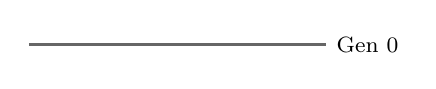
\begin{tikzpicture}[scale=0.42, thick]
  \draw[color=black!60] (0,0) -- (9,0) node[right,black]{\footnotesize Gen 0};
\end{tikzpicture}
\quad
\begin{tikzpicture}[scale=0.42, thick]
  \draw (0,0) -- (3,0) -- (3,3) -- (6,3) -- (6,0) -- (9,0);
  \node[right] at (9,0) {\footnotesize Gen 1 (5 segs)};
\end{tikzpicture}
\end{center}
\begin{answerbox}
\textbf{3rd generation} = apply the same 5-segment rule to \emph{each} of the 5 segments of generation 1 (i.e.\ 2 recursive applications from the base line) $\Rightarrow 5\times5=25$ segments:
\begin{center}
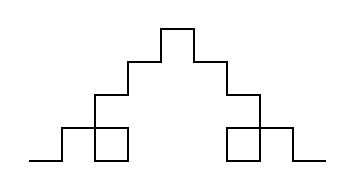
\begin{tikzpicture}[scale=0.42, thick]
\draw plot coordinates {
(0.000,0.000) (1.000,0.000) (1.000,1.000) (2.000,1.000) (2.000,0.000)
(3.000,0.000) (3.000,1.000) (2.000,1.000) (2.000,2.000) (3.000,2.000)
(3.000,3.000) (4.000,3.000) (4.000,4.000) (5.000,4.000) (5.000,3.000)
(6.000,3.000) (6.000,2.000) (7.000,2.000) (7.000,1.000) (6.000,1.000)
(6.000,0.000) (7.000,0.000) (7.000,1.000) (8.000,1.000) (8.000,0.000)
(9.000,0.000)
};
\end{tikzpicture}
\end{center}
\end{answerbox}

%=====================================================================
\section{Examination 2022 --- Q2(a--d) (Section A)}
%=====================================================================
\begin{solutionbox}
\textbf{Question breakdown:}
\begin{enumerate}[noitemsep]
  \item[(a)] What do you mean by the 8-way symmetry of a circle? Explain with a diagram. (1.5)
  \item[(b)] Indicate raster locations chosen by the Midpoint circle algorithm for radius $10$, center $(50,50)$. (4)
  \item[(c)] Why do slanted lines look comparatively dimmer than straight lines? How do you solve this? (2)
  \item[(d)] A type of Koch curve is drawn from a triangle to a 6-pointed star (1st/2nd generation). Draw the 3rd generation. (1.5)
\end{enumerate}
\end{solutionbox}

\subsection*{Q2(a) --- 8-Way Symmetry [1.5 marks]}
See \S1.2. One computed point $(x,y)$ in the $90°$--$45°$ octant yields 7 more by reflecting about the axes and the $45°$ diagonal: $(x,y),(y,x),(-y,x),(-x,y),(-x,-y),(-y,-x),(y,-x),(x,-y)$.

\subsection*{Q2(b) --- Midpoint Circle, $r=10$, Center $(50,50)$ [4 marks]}
\begin{solutionbox}
Octant trace relative to the origin is identical to \S3's table above (same $r=10$): $(0,10),(1,10),(2,10),(3,10),(4,9),(5,9),(6,8),(7,7)$.
\end{solutionbox}
\begin{answerbox}
Apply 8-way symmetry, then \textbf{translate every point by $(+50,+50)$} (i.e.\ replace setPixel$(x,y)$ with setPixel$(x{+}50,y{+}50)$). E.g.\ octant points become
$$(50,60),(51,60),(52,60),(53,60),(54,59),(55,59),(56,58),(57,57)$$
and the remaining 48 points of the full 56-point circle are the 7 symmetric reflections of each, each likewise shifted by $(+50,+50)$.
\end{answerbox}

\subsection*{Q2(c) --- Why Dimmer + How to Fix [2 marks]}
\begin{answerbox}
\textbf{Why:} see \S1.4 --- diagonal pixel spacing ($\sqrt2$ units) vs.\ axis-aligned spacing (1 unit) at equal intensity $\Rightarrow$ lower perceived density $\Rightarrow$ dimmer. \textbf{Fix:} apply an \textbf{anti-aliasing} technique --- e.g.\ \emph{area sampling} (weight each pixel by \% overlap with the true line) or \emph{super-sampling} (subdivide into subpixels, intensity $\propto$ fraction covered) --- to boost the slanted line's pixels proportionally so its perceived brightness matches a horizontal/vertical line of the same true intensity.
\end{answerbox}

\subsection*{Q2(d) --- Koch Curve, 3rd Generation (Triangle $\to$ Star) [1.5 marks]}
\begin{solutionbox}
Gen 1 (given) = equilateral triangle, 3 segments. Gen 2 (given) = classic Koch rule applied once per edge $\Rightarrow 3\times4=12$ segments (the 6-pointed star / hexagram).
\end{solutionbox}
\begin{center}
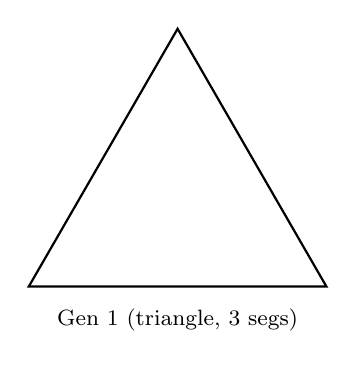
\begin{tikzpicture}[scale=0.42, thick]
  \draw (0,0)--(9,0)--(4.5,7.794)--cycle;
  \node at (4.5,-1) {\footnotesize Gen 1 (triangle, 3 segs)};
\end{tikzpicture}
\quad
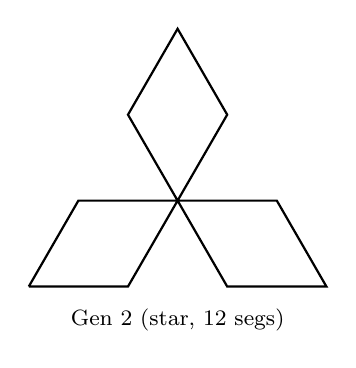
\begin{tikzpicture}[scale=0.42, thick]
\draw plot coordinates {(0.000,0.000) (3.000,0.000) (4.500,2.598) (6.000,0.000) (9.000,0.000) (7.500,2.598) (4.500,2.598) (6.000,5.196) (4.500,7.794) (3.000,5.196) (4.500,2.598) (1.500,2.598) (0.000,0.000)};
\node at (4.5,-1) {\footnotesize Gen 2 (star, 12 segs)};
\end{tikzpicture}
\end{center}
\begin{answerbox}
\textbf{3rd generation} = apply the Koch rule again to \emph{each} of the star's 12 segments $\Rightarrow 3\times16=48$ segments:
\begin{center}
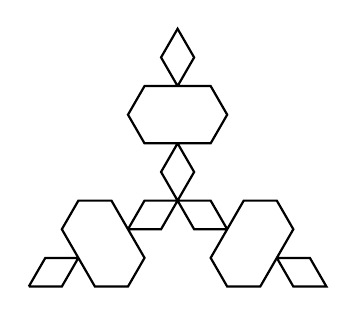
\begin{tikzpicture}[scale=0.42, thick]
\draw plot coordinates {
(0.000,0.000) (1.000,0.000) (1.500,0.866) (2.000,0.000) (3.000,0.000) (3.500,0.866) (3.000,1.732) (4.000,1.732) (4.500,2.598) (5.000,1.732) (6.000,1.732) (5.500,0.866) (6.000,0.000) (7.000,0.000) (7.500,0.866) (8.000,0.000) (9.000,0.000)
(8.500,0.866) (7.500,0.866) (8.000,1.732) (7.500,2.598) (6.500,2.598) (6.000,1.732) (5.500,2.598) (4.500,2.598) (5.000,3.464) (4.500,4.330) (5.500,4.330) (6.000,5.196) (5.500,6.062) (4.500,6.062) (5.000,6.928) (4.500,7.794)
(4.000,6.928) (4.500,6.062) (3.500,6.062) (3.000,5.196) (3.500,4.330) (4.500,4.330) (4.000,3.464) (4.500,2.598) (3.500,2.598) (3.000,1.732) (2.500,2.598) (1.500,2.598) (1.000,1.732) (1.500,0.866) (0.500,0.866) (0.000,0.000)
};
\end{tikzpicture}
\end{center}
(This is the classic \textbf{Koch snowflake}, iteration 2.)
\end{answerbox}

%=====================================================================
\section{Examination 2021 --- Q1(f), Q2(a--b) (Section A)}
%=====================================================================
\begin{solutionbox}
\textbf{Question breakdown:}
\begin{enumerate}[noitemsep]
  \item[Q1(f)] A Quadratic Koch curve: generation 0 = straight line, generation 1 = square bump (shown). Draw generation 2. (1)
  \item[Q2(a)] Line from $(1,1)$ to $(10,7)$: (i) raster locations via basic line algorithm; (ii) why is scan conversion slower than expected; (iii) how Bresenham overcomes this; (iv) raster locations via Bresenham. (1.5+1+1+2.5)
  \item[Q2(b)] Three major adverse effects of scan conversion? Apply the given lowpass filter kernel to the given $5\times5$ pixel grid. (2.75)
\end{enumerate}
\end{solutionbox}

\subsection*{Q1(f) --- Quadratic Koch Curve, Generation 2 [1 mark]}
\begin{answerbox}
Identical construction to 2023 Q2(d) above (same square-bump rule, one generation number lower on this year's labeling): apply the 5-segment square-bump rule to each of generation 1's 5 segments $\Rightarrow$ \textbf{25 segments} (same 26-point coordinate list shown in \S3).
\end{answerbox}

\subsection*{Q2(a) --- Line $(1,1)\to(10,7)$: Basic Algorithm vs.\ Bresenham [6 marks]}
$\Delta x=9,\Delta y=6\Rightarrow m=2/3\approx0.667$ ($|m|\le1$).

\textbf{(i) Basic (direct equation) algorithm} --- $b=y_1-mx_1=1-\frac23=\frac13$; compute $y=\frac23x+\frac13$ and round for each integer $x$:
\begin{answerbox}
$$(1,1),(2,2),(3,2),(4,3),(5,4),(6,4),(7,5),(8,6),(9,6),(10,7)$$
\end{answerbox}

\textbf{(ii) Why slower than expected:} the direct equation requires a floating-point \textbf{multiply} ($mx$) and a \textbf{round/floor} operation at every single step --- expensive compared to simple integer addition.

\textbf{(iii) How Bresenham fixes it:} replaces the per-step multiply with an integer decision variable updated purely by addition/subtraction (see \S1.1) --- no floating-point arithmetic at all.

\textbf{(iv) Bresenham trace:} $\mathrm{Inc}_1=2\Delta y=12$, $\mathrm{Inc}_2=2(\Delta y-\Delta x)=2(6-9)=-6$, $d_1=\mathrm{Inc}_1-\Delta x=12-9=3$.
\begin{solutionbox}
\begin{center}
\begin{tabular}{ccccl}
\toprule
$d$ & $x$ & $y$ & rule \\
\midrule
3  & 1 & 1 & start \\
3  & 2 & 2 & $d>0\Rightarrow d{+}{=}{-}6\Rightarrow{-}3$, $y{+}{+}$ \\
$-3$ & 3 & 2 & $d\le0\Rightarrow d{+}{=}12\Rightarrow9$, same $y$ \\
9  & 4 & 3 & $d>0\Rightarrow d{+}{=}{-}6\Rightarrow3$, $y{+}{+}$ \\
3  & 5 & 4 & $y{+}{+}\Rightarrow d{=}{-}3$ \\
$-3$ & 6 & 4 & same $y\Rightarrow d{=}9$ \\
9  & 7 & 5 & $y{+}{+}\Rightarrow d{=}3$ \\
3  & 8 & 6 & $y{+}{+}\Rightarrow d{=}{-}3$ \\
$-3$ & 9 & 6 & same $y\Rightarrow d{=}9$ \\
9  & 10 & 7 & $y{+}{+}$ \\
\bottomrule
\end{tabular}
\end{center}
\end{solutionbox}
\begin{answerbox}
$$(1,1),(2,2),(3,2),(4,3),(5,4),(6,4),(7,5),(8,6),(9,6),(10,7)$$
Identical to the correctly-rounded basic-algorithm result in (i) --- as expected, since Bresenham is just an efficient reformulation of "pick the nearest pixel to the true line," not a different rule.
\end{answerbox}

\subsection*{Q2(b) --- Three Adverse Effects + Lowpass Filter [2.75 marks]}
\begin{answerbox}
\textbf{Three adverse effects:} staircase/jaggies, unequal brightness of slanted lines, the picket fence problem (see \S1.4).
\end{answerbox}
\textbf{Lowpass filtering:} new value $=\sum(\text{kernel weight})\times(\text{corresponding original pixel value})$, kernel centered on each pixel. For the given $3\times3$ kernel (top neighbor weight $3$, bottom neighbor weight $2$, all else $0$) applied to the interior of the given $5\times5$ grid:
\begin{solutionbox}
$$\text{new}(r,c) = 3\times\text{grid}(r{-}1,c) + 2\times\text{grid}(r{+}1,c)$$
\begin{center}
\begin{tabular}{ccc}
$3(0)+2(25)=\mathbf{50}$ & $3(0)+2(92)=\mathbf{184}$ & $3(0)+2(31)=\mathbf{62}$ \\
$3(13)+2(44)=\mathbf{127}$ & $3(31)+2(74)=\mathbf{241}$ & $3(46)+2(94)=\mathbf{326}$ \\
$3(25)+2(0)=\mathbf{75}$ & $3(92)+2(0)=\mathbf{276}$ & $3(31)+2(0)=\mathbf{93}$ \\
\end{tabular}
\end{center}
\end{solutionbox}
\begin{notesbox}
\textbf{Method is what's graded, not these exact numbers} --- re-read the kernel and grid values off your own copy of the paper before the exam; the mechanical rule (multiply-and-sum a centered kernel over the neighborhood) is what must be memorised.
\end{notesbox}

%=====================================================================
\section{Examination 2020 --- Q2(d), Q3(b--c), Q4(c) (Group-A)}
%=====================================================================
\begin{solutionbox}
\textbf{Question breakdown:}
\begin{enumerate}[noitemsep]
  \item[Q2(d)] Could you fill the given arrow shape using the Flood-Fill algorithm with 8-connected pixels? Justify. (2.5)
  \item[Q3(b)] Show raster locations while drawing a line using DDA from $(1,1)$ to $(5,8)$. (3.75)
  \item[Q3(c)] Find raster locations using Bresenham's algorithm, line from $(0,0)$ to $(8,5)$. (4)
  \item[Q4(c)] Show 8-way symmetry of a circle. (1)
\end{enumerate}
\end{solutionbox}

\subsection*{Q2(d) --- Flood-Fill an Arrow, 8-Connected [2.5 marks]}
\begin{answerbox}
Same reasoning as 2023 Q2(c) (\S3): an arrow shape has slanted edges (the head's diagonal sides), so its scan-converted boundary is a single-pixel staircase that is only 4-connected along its length. Running \textbf{flood-fill with 8-connected} logic lets the fill step diagonally through the corner-gaps in that staircase, \textbf{leaking out of the arrow at its diagonal edges} --- so no, it cannot be reliably filled this way without first thickening the boundary or switching the fill to 4-connected.
\end{answerbox}

\subsection*{Q3(b) --- DDA, $(1,1)\to(5,8)$ [3.75 marks]}
$\Delta x=4,\Delta y=7\Rightarrow m=7/4=1.75$ ($|m|>1$, so step $y$ by 1, $x_{i+1}=x_i+1/m=x_i+4/7$).
\begin{solutionbox}
\begin{center}
\begin{tabular}{cccc}
\toprule
$y$ & $x$ (exact) & pixel $x$ & pixel \\
\midrule
1 & 1.000 & 1 & $(1,1)$ \\
2 & 1.571 & 2 & $(2,2)$ \\
3 & 2.143 & 2 & $(2,3)$ \\
4 & 2.714 & 3 & $(3,4)$ \\
5 & 3.286 & 3 & $(3,5)$ \\
6 & 3.857 & 4 & $(4,6)$ \\
7 & 4.429 & 4 & $(4,7)$ \\
8 & 5.000 & 5 & $(5,8)$ \\
\bottomrule
\end{tabular}
\end{center}
\end{solutionbox}
\begin{answerbox}
$$(1,1),(2,2),(2,3),(3,4),(3,5),(4,6),(4,7),(5,8)$$
\end{answerbox}

\subsection*{Q3(c) --- Bresenham, $(0,0)\to(8,5)$ [4 marks]}
$\Delta x=8,\Delta y=5\Rightarrow m=0.625$ ($0<m<1$). $\mathrm{Inc}_1=2\Delta y=10$, $\mathrm{Inc}_2=2(\Delta y-\Delta x)=2(5-8)=-6$, $d_1=\mathrm{Inc}_1-\Delta x=10-8=2$.
\begin{solutionbox}
\begin{center}
\begin{tabular}{cccl}
\toprule
$d$ & $x$ & $y$ & rule \\
\midrule
2 & 0 & 0 & start \\
2 & 1 & 1 & $d>0\Rightarrow d{+}{=}{-}6\Rightarrow{-}4$, $y{+}{+}$ \\
$-4$ & 2 & 1 & $d\le0\Rightarrow d{+}{=}10\Rightarrow6$, same $y$ \\
6 & 3 & 2 & $d>0\Rightarrow d{+}{=}{-}6\Rightarrow0$, $y{+}{+}$ \\
0 & 4 & 2 & $d\le0\Rightarrow d{+}{=}10\Rightarrow10$, same $y$ \\
10 & 5 & 3 & $d>0\Rightarrow d{+}{=}{-}6\Rightarrow4$, $y{+}{+}$ \\
4 & 6 & 4 & $d>0\Rightarrow d{+}{=}{-}6\Rightarrow{-}2$, $y{+}{+}$ \\
$-2$ & 7 & 4 & $d\le0\Rightarrow d{+}{=}10\Rightarrow8$, same $y$ \\
8 & 8 & 5 & $y{+}{+}$ \\
\bottomrule
\end{tabular}
\end{center}
\end{solutionbox}
\begin{answerbox}
$$(0,0),(1,1),(2,1),(3,2),(4,2),(5,3),(6,4),(7,4),(8,5)$$
\end{answerbox}

\subsection*{Q4(c) --- 8-Way Symmetry of a Circle [1 mark]}
See \S1.2 --- one octant point $(x,y)$ mirrors to 7 others: $(x,y),(y,x),(-y,x),(-x,y),(-x,-y),(-y,-x),(y,-x),(x,-y)$.

%=====================================================================
\section{Quick Summary --- Exam Patterns for Chapter 3}
%=====================================================================

\begin{center}
\renewcommand{\arraystretch}{1.3}
\begin{tabular}{p{5cm}|p{2.7cm}|p{6.3cm}}
\toprule
\textbf{Pattern} & \textbf{Years} & \textbf{Method to memorise} \\
\midrule
DDA vs.\ Bresenham line trace & 2020, 2021, 2024 & Table walk: DDA rounds $y{+}{=}m$ each step; Bresenham updates integer $d$ by $\mathrm{Inc}_1$ or $\mathrm{Inc}_2$ \\
Bresenham/DDA conceptual (why faster) & 2021, 2023 & No floating multiply/round in Bresenham; integer add/shift only \\
Midpoint circle raster trace (octant + symmetry) & 2022, 2023 & $p_1=1{-}r$; $p<0\Rightarrow p{+}{=}2x{+}3$; else $p{+}{=}2(x{-}y){+}5,\,y{-}{-}$ \\
8-way symmetry (theory only) & 2020, 2022 & {\scriptsize $(x,y),(y,x),(-y,x),(-x,y),(-x,-y),(-y,-x),(y,-x),(x,-y)$} \\
Slanted-line dimness (why / how to fix) & 2021, 2022, 2023 & $\sqrt2$ vs.\ 1 unit pixel spacing; fix via area/super-sampling anti-aliasing \\
Flood-fill 4/8-connected leak reasoning & 2020, 2023 & Same connectivity for boundary \& fill is self-contradictory on diagonal edges \\
Koch curve, draw next generation & 2021, 2022, 2023 & Square-bump: $\times5$ segs/edge/iter; classic triangular: $\times4$ segs/edge/iter \\
\bottomrule
\end{tabular}
\end{center}

\begin{notesbox}
\textbf{Exam-day strategy for the Scan Conversion cluster:} this question is entirely mechanical once the two decision-variable recurrences (line, circle) are memorised cold --- there is no derivation required in the exam, only correct step-by-step table execution. Budget the marks accordingly: a full trace (line or circle) is usually worth 3--4 marks for maybe 8--10 minutes of careful arithmetic; the conceptual sub-parts (why dimmer, why Bresenham is faster, flood-fill leak reasoning) are 1--2 mark free points if the one-line reasons above are memorised.
\end{notesbox}

\end{document}
